\FloatBarrier

\begin{figure}[h!]
	\centering
	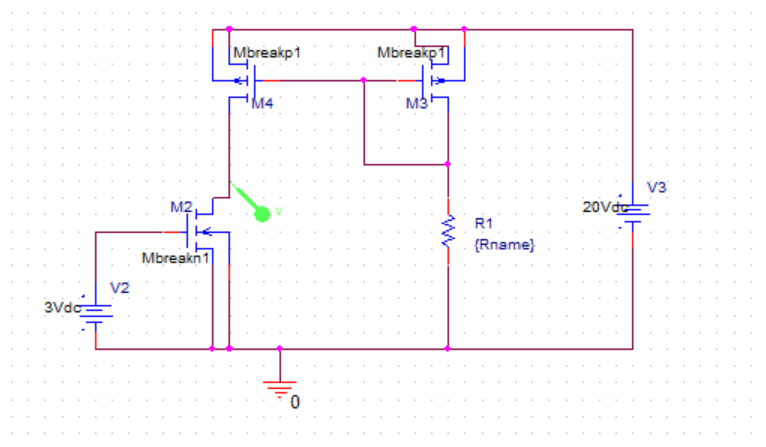
\includegraphics[scale=0.75]{../images/circuit5.PNG}
	\caption{Common Source Amplifier with Complementary Load}
	\label{fig:circuit5}
\end{figure}

\FloatBarrier

\FloatBarrier

\begin{figure}[h!]
	\centering
	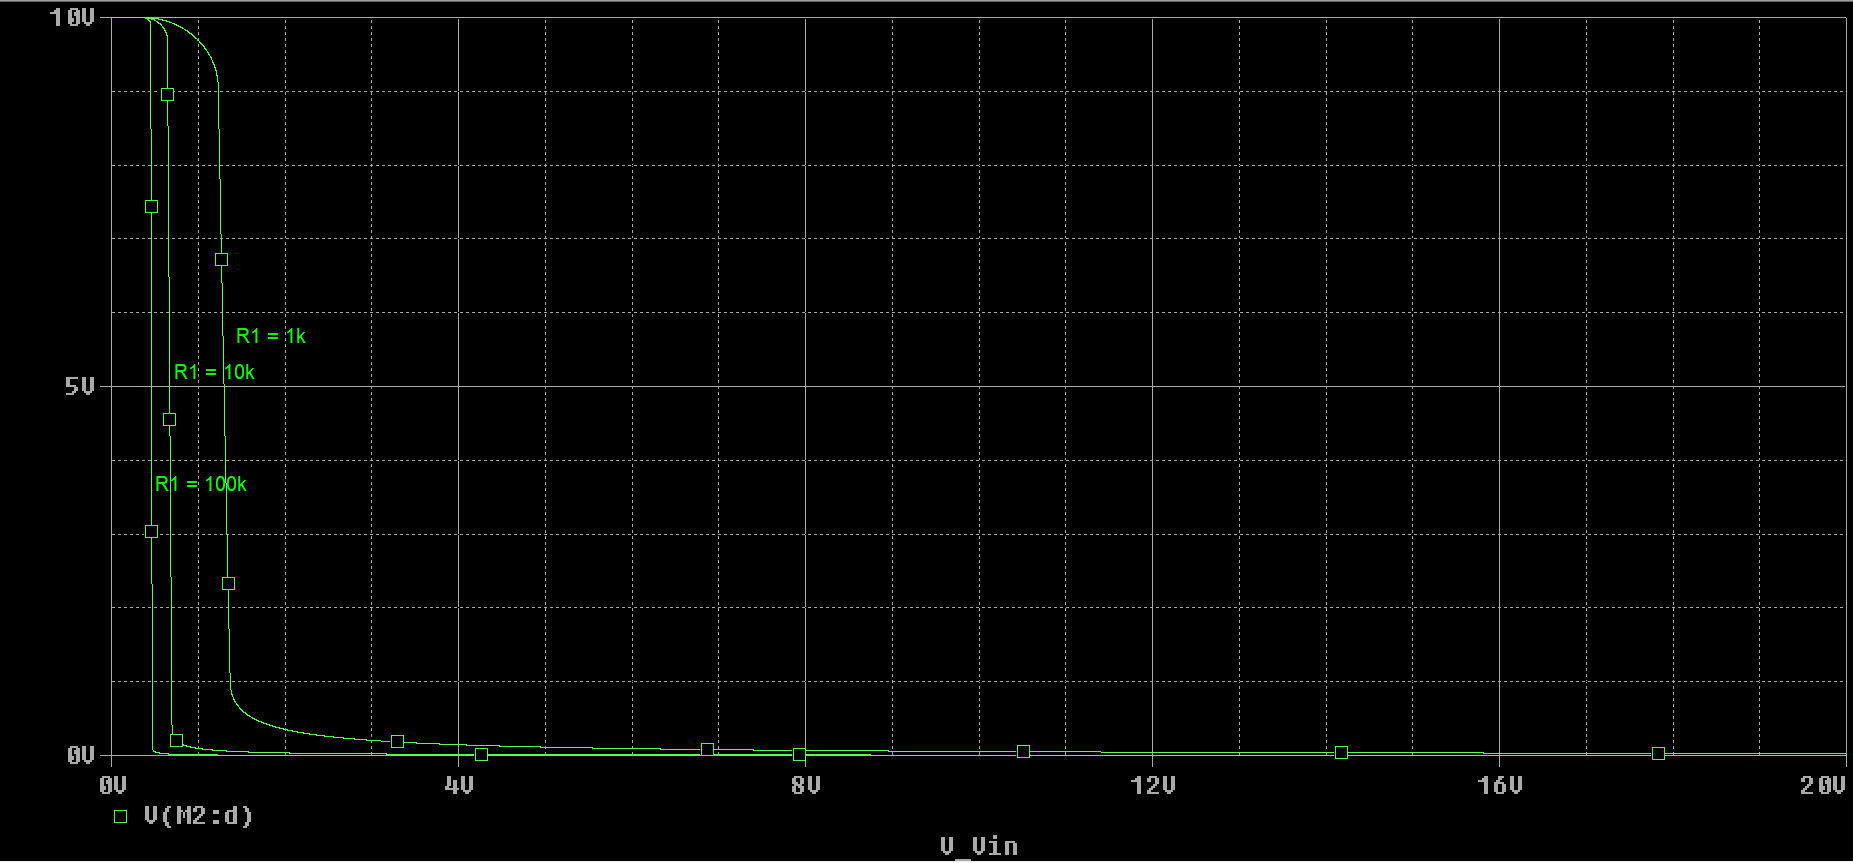
\includegraphics[scale=0.75]{../images/dc_sweep_vin.PNG}
	\caption{Voltage Transfer Characteristic}
	\label{fig:dc_sweep_vin}
\end{figure}

\FloatBarrier

\FloatBarrier

\begin{figure}[h!]
	\centering
	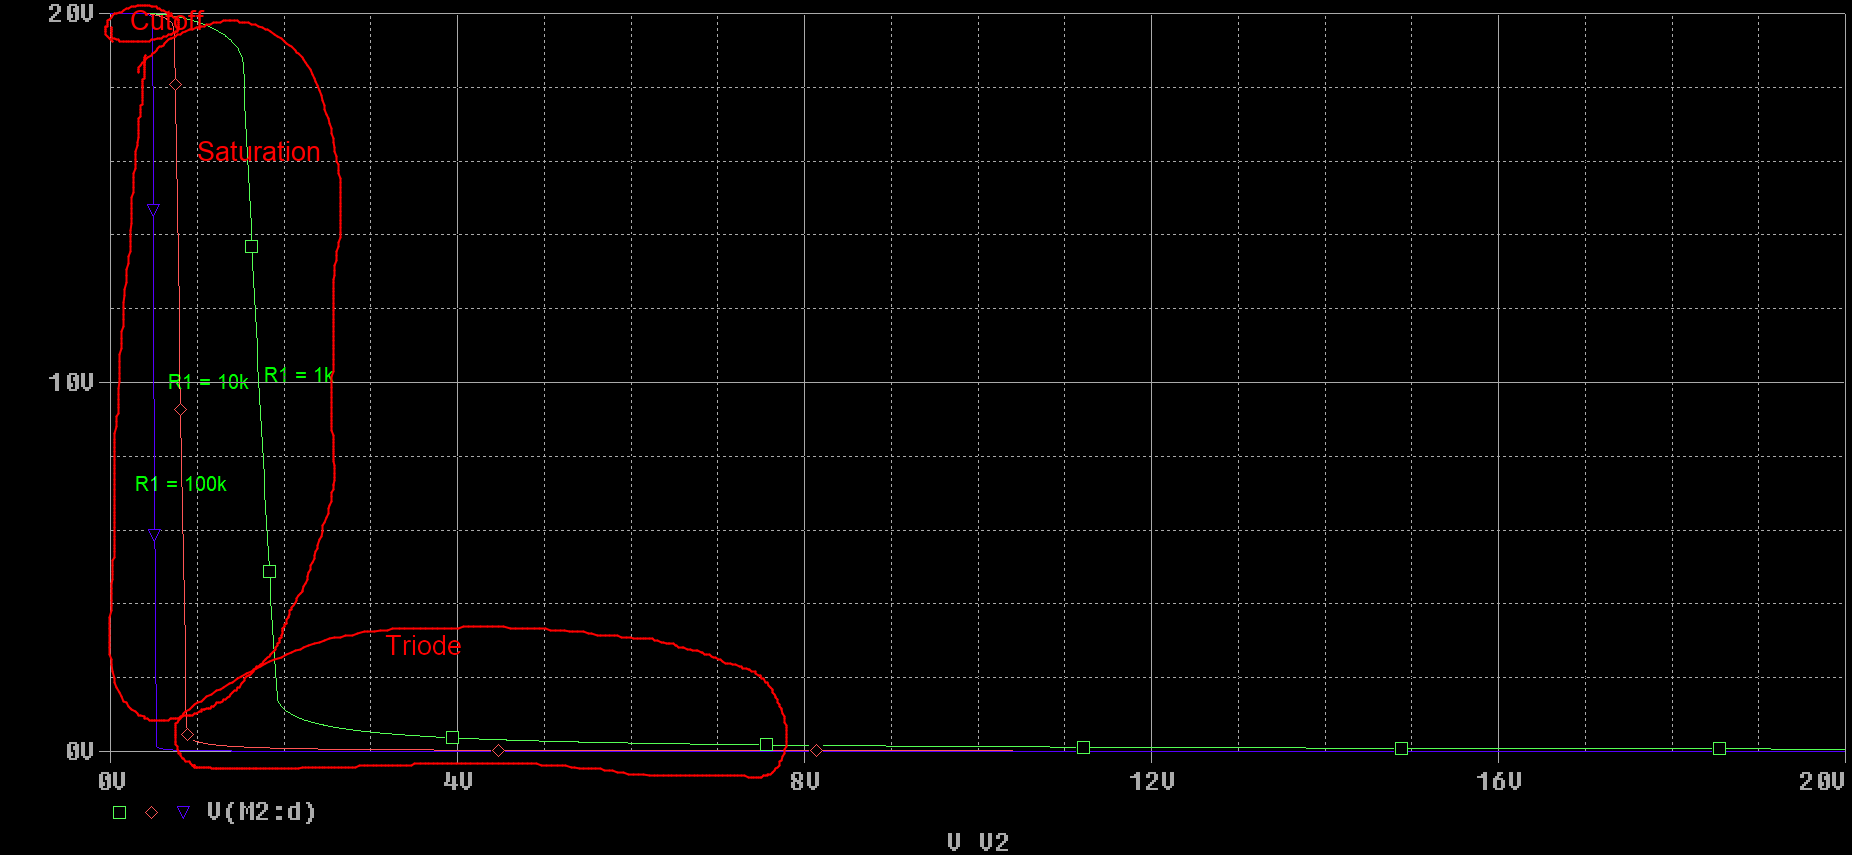
\includegraphics[scale=0.75]{../images/dc_sweep_vin_labeled.PNG}
	\caption{Voltage Transfer Characteristic with Regions of Operation}
	\label{fig:dc_sweep_vin_labeled}
\end{figure}

\FloatBarrier

% Find gain
The gain can be approximated by calculating the slope of the curve in the saturation region given two points. For $R_1 = 1$\si{\kilo\ohm}, the gain is approximately $-58 \frac{V}{V}$. For $R_1 = 10$\si{\kilo\ohm}, the gain is approximately $-170 \frac{V}{V}$. For $R_1 = 100$\si{\kilo\ohm}, the gain is approximately $-507 \frac{V}{V}$. \\

\FloatBarrier

\begin{table}[h!]
	\centering
	\caption{Voltage Gain at Different $R_1$ Values}
	\label{tab:gain}
	\csvautotabular{../tables/gain.csv}
\end{table}

\FloatBarrier

% Pick R value for bias
Again, the best resistor value is the one that leads to the steepest descent, or equivalently highest gain, in the saturation region. This occurs when the load is largest. So, $R_1 = 100$\si{\kilo\ohm} is the best choice for a good voltage amplifier and inverter. \\
